\section{Ergebnisse}


\subsection{Implementierung des Frontends}

\begin{itemize}
	\item Tools
	\begin{itemize}
	
		\item TypeScript
		\begin{itemize}
			\item Typ-Sichere version von JavaScript
			\item Compiliert auf JavaScript
		\end{itemize}
		
		\item npm
		\begin{itemize}
			\item Three.js als dependency
			\item AR.js von github
			\begin{itemize}
				\item TypeScript declaration file
			\end{itemize}
		\end{itemize}
		
		\item webpack
	\end{itemize}
	
	\item Workflow + Klassen + Funktionen + Sequenz-Diagramm
	
	\item GUI
	\begin{itemize}
		\item Spannt eine GUI ebene auf mit der sich eine ebene zum Filtern der Vektor daten aktivieren und einstellen lässt
		\item Triggert gewisse Events, bei Änderungen
		\begin{itemize}
			\item Wird genutzt um Filer an zu passen
		\end{itemize}
		\item Daten werden bei anfrage an Backend genutzt
	\end{itemize}
\end{itemize}



\subsection{Implementierung des Backends}

\begin{figure}[H]
	\centering
	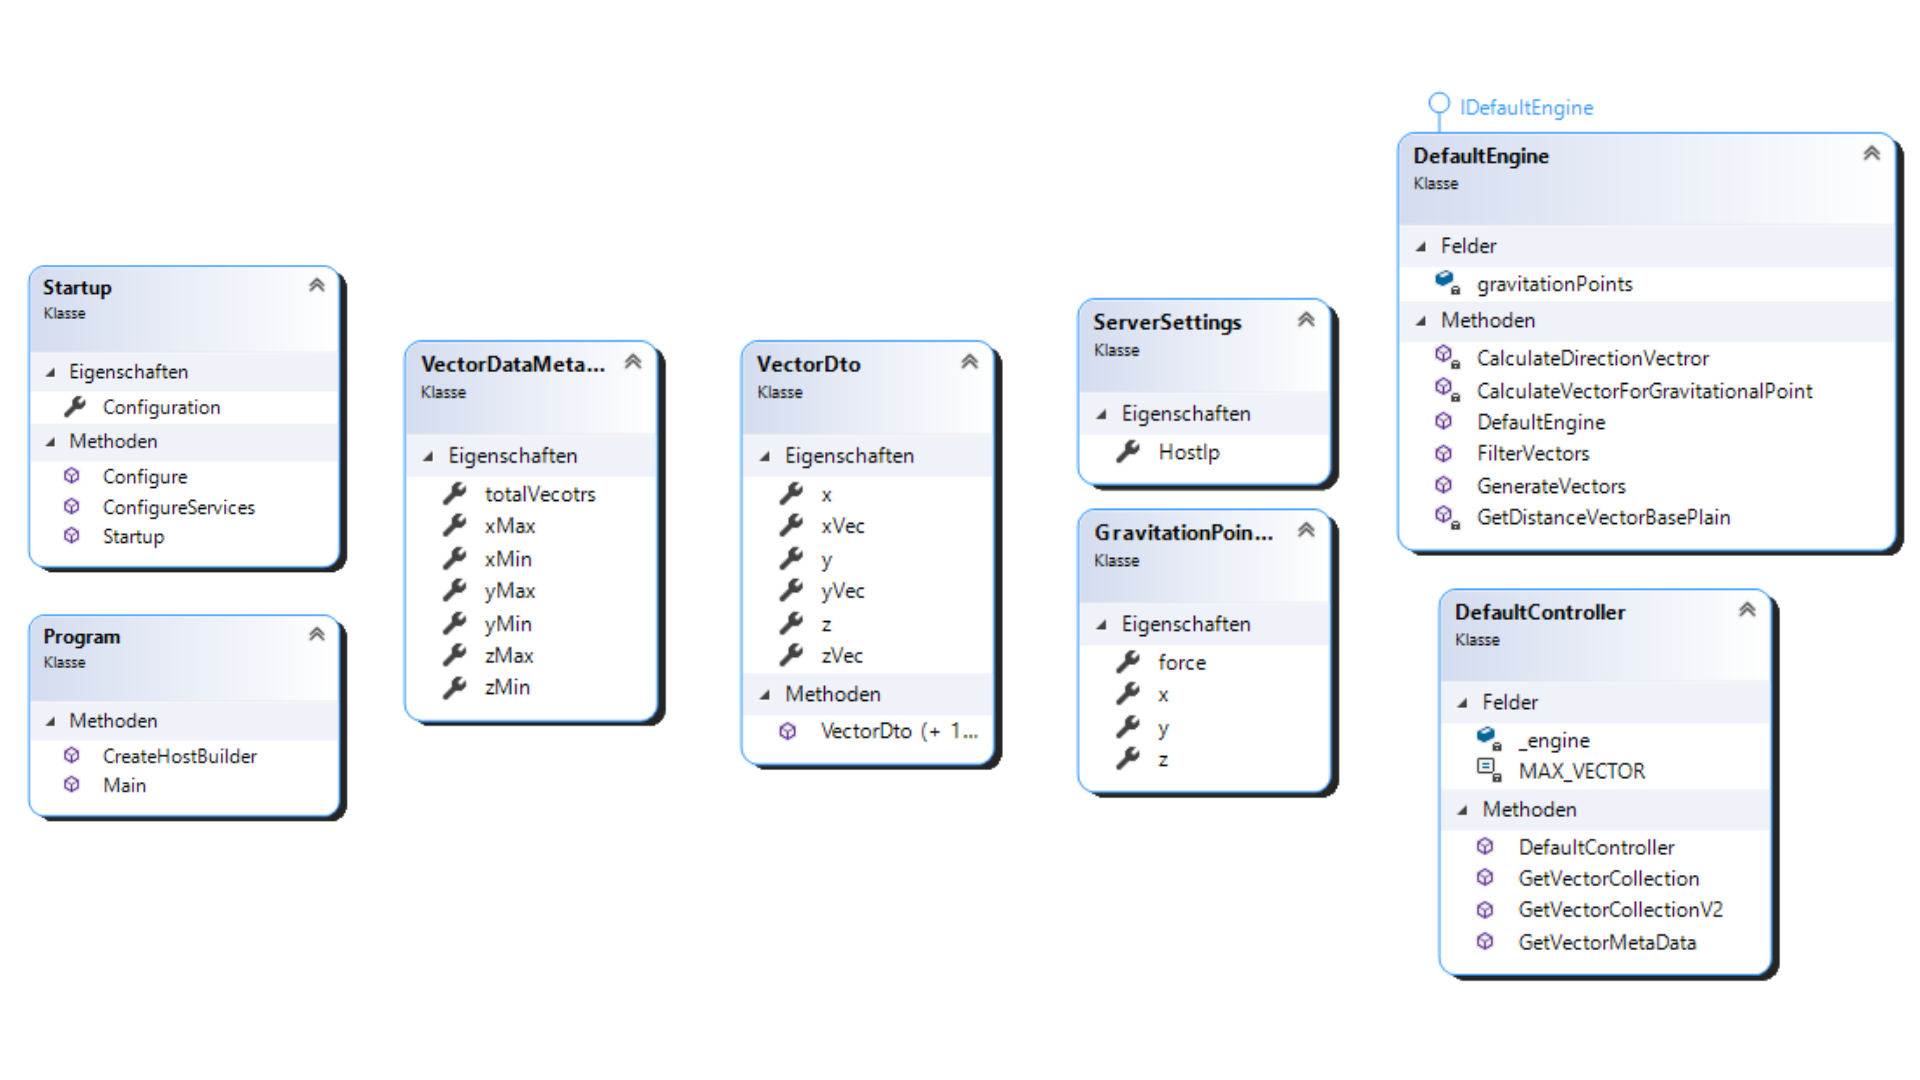
\includegraphics[width=\linewidth]{images/backend/classDiagram}
	\caption{System Klassen, Dto Klassen und Controller und Engine Klassen}
	\label{fig:ClassDiagram}
\end{figure}

Die Backend API wird in Asp.NetCore (C\#) implementiert.
Das Framework wurde gewählt, da es kostenlos und opensource
ist und da es sowohl auf Linux als auch auf Windows lauffähig ist
(vgl. DotNet Download page \cite{DotNetDownloadPage}).
Außerdem liefert NetCore mit ASP nativ eine IIS Webapplikation
Funktionalität mit, sodass die API schnell und einfach umzusetzen ist,
ohne einen großen web hosting Overhead zu erzeugen. Grundsätzlich
besteht das Programm aus drei Klassen Gruppen, den System Klassen,
den Controller und Engine Klassen und den Daten Transfer Objekt (Dto)
Klassen (siehe Abbildung \ref{fig:ClassDiagram}).

Die Klasse Programm besitzt vordefinierten code zur Instanziierung
des WebHosts. Um Die Host Ip selbst festlegen zu können wurde dieser
Code um die ServerSettings erweitert, welche die HostIp aus der
apsettings.json bezieht
(Code \ref{code:Program.cs}:\ref{line:SettingsBind}) und im
CreateHostBuilder diese als HostURL verwendet
(Code \ref{code:Program.cs}:\ref{line:HostURL}).

\begin{codeblock}
	\begin{lstlisting}[
		style=sharpc,
		caption={Methoden der Program Klasse},
		label={code:Program.cs}
	]
public static void Main(string[] args)
{
	var config = new ConfigurationBuilder()
		.AddJsonFile("appsettings.json", optional: false)
		.Build();
	var serSet = new ServerSettings();
	config.GetSection("ServerSettings").Bind(serSet); `\label{line:SettingsBind}`
	CreateHostBuilder(args, serSet).Build().Run();
}

public static IHostBuilder CreateHostBuilder(string[] args, ServerSettings serverSettings) =>
	Host.CreateDefaultBuilder(args)
		.ConfigureWebHostDefaults(webBuilder =>
		{
			webBuilder.UseStartup<Startup>();
			webBuilder.UseUrls(serverSettings.HostIp); `\label{line:HostURL}`
		});
	\end{lstlisting}
\end{codeblock}

In der zweiten Systemklassen \grqq Startup.cs\grqq\space werden die
Webhost und Umgebungseinstellungen getätigt.
In Code \ref{code:ConfigureServices} Zeile \ref{line:ApplyConfig}
wird der Teil \grqq AppSettings\grqq\space aus der
\grqq appsettings.json\grqq\space ausgelesen und in die Dto Klasse
\grqq AppSettings\grqq\space geparsed. Diese Instanz wird dann
mithilfe von Dependency injection an alle Instanzen verteilt,
welche das Objekt benötigen. In den Zeilen \ref{line:CorsPolicyStart}
- \ref{line:CorsPolicyEnd} wird für später die CORS Policy definiert.
Die hier definierte Policy wird jede Origin, mit jeder HTTP Methode
und jedem Header akzeptieren. Außerdem wird in Zeile
\ref{line:DefaultEngineV2Singleton} eine Instanz von DefaultEngineV2
als Singleton für IDefaultEngine via Dependancy Injection definiert.
Dependency Injection wird verwendet um ein einfaches austauschen der
Engine zu ermöglichen und zur Vereinfachung des Lifetimemanagement
der DefaultEngineV2 Instanz im DefaultController.

\begin{codeblock}
	\begin{lstlisting}[
		style=sharpc,
		caption={Methode ConfigureServices in Startup.cs},
		label={code:ConfigureServices}
	]
public void ConfigureServices(IServiceCollection services)
{
	services.Configure<AppSettings>(Configuration.GetSection("AppSettings"));	`\label{line:ApplyConfig}`
	services.AddCors(o => o.AddPolicy("AllowAnyOrigin", builder => { `\label{line:CorsPolicyStart}`
		builder.AllowAnyOrigin()
			.AllowAnyMethod()
			.AllowAnyHeader();
	})); `\label{line:CorsPolicyEnd}`
	services.AddSingleton<IDefaultEngine, DefaultEngineV2>(); `\label{line:DefaultEngineV2Singleton}`
	services.AddControllers();
	services.AddDirectoryBrowser();
}
	\end{lstlisting}
\end{codeblock}

Diese Methode wird zu Laufzeit vor Configure
(Code \ref{code:Configure}) aufgerufen. In Configure werden nun
einige wichtige Einstellungen getätigt. In Code \ref{code:Configure}
Zeile \ref{line:UseCors} wird die vorher in ConfigureServices definierte
\grqq AllowAnyOrigin\grqq -Policy für die ganze WebApp übernommen.
In den Zeilen \ref{line:StaticFilesStart} - \ref{line:StaticFilesEnd}
wird eingestellt welche statischen Dateien gehostet werden sollen,
wo diese liegen und wo diese aufzufinden sein sollen. So wird nun
der gesamte Inhalt des Ordners wwwroot am /data Endpunkt zur
Verfügung gestellt. Der zuvor erstellte FileExtensionContentTypeProvider
(Code \ref{code:Configure}:
\ref{line:FileExtensionContentTypeProviderStart} -
\ref{line:FileExtensionContentTypeProviderEnd})
definiert mit welchem Content-Type Header die "unbekannten"
Datentypen übermittelt werden sollen. Wenn keine eindeutige
Definition vorliegt wird die Datei mit dem Standard Header
"text/html" nur dann ausgeliefert wenn ServeUnknowFileTypes auf
true gesetzt wurde.
Asp.NetCore liefert von sich einen Directory Browser mit,
welcher eine graphische UI zur Navigation durch die statischen
Dateien generiert (siehe Abbildung \ref{fig:DirectoryBrowser}).
Dieser wird in Zeile \ref{line:UseDirectoryBrowser} aktiviert.
Die letzten Zeilen sind von Asp.NetCore für API Anwendungen
standardmäßig generierte Codezeilen. Sie aktivieren das Standard
Routing und definieren die Controller als verarbeitende Endpunkte.

\begin{codeblock}
	\begin{lstlisting}[
		style=sharpc,
		caption={Methode Configure in Startup.cs},
		label={code:Configure}
	]
public void Configure(IApplicationBuilder app, IWebHostEnvironment env)
{
	app.UseCors("AllowAnyOrigin"); `\label{line:UseCors}`

	var provider = new FileExtensionContentTypeProvider(); `\label{line:FileExtensionContentTypeProviderStart}`
	provider.Mappings[".dat"] = "application/octet-stream";
	provider.Mappings[".patt"] = "text/html";
	provider.Mappings[".mtl"] = "text/html";
	provider.Mappings[".obj"] = "text/html"; `\label{line:FileExtensionContentTypeProviderEnd}`

	app.UseStaticFiles(new StaticFileOptions `\label{line:StaticFilesStart}`
	{
		ServeUnknownFileTypes=true,
		FileProvider = new PhysicalFileProvider(Path.Combine(env.WebRootPath, "data")),
		RequestPath = "/data",
		ContentTypeProvider = provider
	}); `\label{line:StaticFilesEnd}`
	app.UseDirectoryBrowser(); `\label{line:UseDirectoryBrowser}`
	app.UseRouting();
	app.UseEndpoints(endpoints =>
	{
		endpoints.MapControllers();
	});
}
	\end{lstlisting}
\end{codeblock}

\begin{figure}
	\centering
	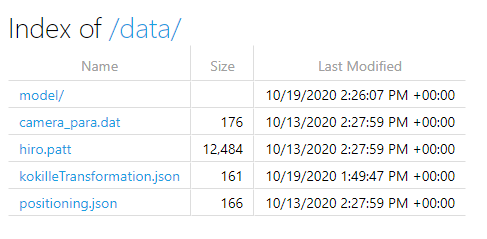
\includegraphics[width=0.7\linewidth]{images/backend/DirectoryBrowser}
	\caption{Directory Browser zur Navigation durch statische Dateien des Servers}
	\label{fig:DirectoryBrowser}
\end{figure}

Bei der ersten anfrage an die API wird eine Instanz des implementierten
Controllers erstellt, welche nun die einkommenden Anfragen verarbeitet.
Der DefaultControler bekommt bei Instanziierung via Dependency Injection
die vorher in ConfigureServices definierte Instanz einer IDefaultEngine
Interface implementierenden Klasse
(vgl. Code \ref{code:DefaultControllerConstructor}).
Diese Aufteilung in Controller und Engine wurde definiert um eine besser
Codeübersicht zu gewährleisten. So ist die input verarbeitende Controller
Klasse von der Datenverarbeitenden Engine Klasse losgelöst.

\begin{codeblock}
	\begin{lstlisting}[
		style=sharpc,
		caption={Konstruktor der DefaultController Klasse},
		label={code:DefaultControllerConstructor}
	]
private IDefaultEngine _engine;

public DefaultController(IDefaultEngine engine)
{
	_engine = engine;
}
	\end{lstlisting}
\end{codeblock}

Die Controller Klasse implementiert die in Kapitel \ref{section:Backend}
Definierten Endpunkte. GetVectorMetaData bezieht die Metadaten mit einem
Methoden Aufruf aus der Engine Klasse und gibt diese dann zurück.
Die GetVectorCollection Methode akzeptiert 8 optionale Parameter
(siehe Tabelle \ref{tab:EndpointQueryParameters}). Aufgrund von API
design best practices (vgl. Narumoto \cite{ApiDesignBestPractices})
und aufgrund von potentiell hoher Datenmenge unterstützt der Endpunkt
pagination. Durch setzen von limit und offset kann so gesteuert werden
wieviele und welche Teile der Vektor Daten zurückgegeben werden.
Durch angeben von n1, n2, n3, x, y, und z können die Ergebnisse
zusätzlich gefiltert werden. Dies geschieht in der Engine Klasse.

\begin{table}
	\centering
	\begin{tabular}[h]{p{0.11\linewidth} | p{0.7\linewidth}| p{0.09\linewidth}}
	Parameter & Beschreibung & Default \\
	\hline
	limit & Limitiert die Anzahl an zurückgegebenen Vectoren & 100\\
	offset & Definiert den Abstand vom ersten zurückgegebenen Vektor zum ersten Vektor im Datensatz & 0\\
	n1 & x-Koordinate des Normalenvektors der Filter-Ebene & null\\
	n2 & y-Koordinate des Normalenvektors der Filter-Ebene & null\\
	n3 & z-Koordinate des Normalenvektors der Filter-Ebene & null\\
	x & x-Koordinate eines punktes auf der Filter-Ebene & null\\
	y & y-Koordinate eines punktes auf der Filter-Ebene & null\\
	z & z-Koordinate eines punktes auf der Filter-Ebene & null\\
	maxDist & Definiert den maximalen Abstand, den ein Punkt von der Filter-Ebene haben darf um zurückgegeben zu werden & 0.5\\
	\end{tabular}
	\caption{Query Parameter des api/data/ Endpunktes}
	\label{tab:EndpointQueryParameters}
\end{table}

Die DefaultEngine Klasse Implementiert, das IDefaultEngine Interface
und mit Ihr auch die Methoden GetAllVectors, GetVectorMetaData,
und FilterVectors. Sie bezieht die AppSettings des Programms via
Dependency Injection (vgl. Code \ref{code:DefaultEngineConstructor}).

\begin{codeblock}
	\begin{lstlisting}[
		style=sharpc,
		caption={Konstruktor der DefaultEngine Klasse},
		label={code:DefaultEngineConstructor}
	]
private AppSettings _settings;

public DefaultEngineV2(IOptions<AppSettings> settings)
{
	_settings = settings.Value;
}
	\end{lstlisting}
\end{codeblock}

Dieses Settings Objekt ist erforderlich, da es den Pfad zu der Datei
beinhaltet, welche die Vektordaten enthält. Dieser Pfad wird von der
Methode \grqq GetAllVectors\grqq\space an die private Methode
\grqq LoadVectorsFromJsonFile\grqq\space weitergegeben, welche
wiederum mithilfe des \grqq StreamReaders\grqq\space zunächst die
Datei einliest und anschließend mit \grqq JsonConvert\grqq\space
in eine Liste an VectorDto Objekten paarst.
(vgl. Code \ref{code:GetAllVectors})

\begin{codeblock}
	\begin{lstlisting}[
		style=sharpc,
		caption={Akquirieren der Vektordaten von einer in den App-Settings definierten Datei},
		label={code:GetAllVectors}
	]
private List<VectorDto> LoadVectorsFromJsonFile(string path)
{
	var returnList = new List<VectorDto>();

	using (StreamReader r = new StreamReader(path))
	{
		string json = r.ReadToEnd();
		returnList = JsonConvert.DeserializeObject<List<VectorDto>>(json);
	}

		return returnList;
	}

public List<VectorDto> GetAllVectors()
{
	return LoadVectorsFromJsonFile(_settings.jsonPath);
}
	\end{lstlisting}
\end{codeblock}

Diese Funktionen werden auch von \grqq GetVectorMetaData\grqq\space
aufgerufen, welche dann jeweils die x,y und z Minima und Maxima und
die Anzahl an Vektoren ermittelt ermittelt. Diese werden dann als
\grqq VectorDataMetaData\grqq\space zurückgegeben.

Die Engine Klasse stellt auch eine FilterVectors Methode zur Verfügung.
Die Methode nimmt einen ein plainVectorDto Objekt, die maximale Distanz
und die zu filternden Vektoren entgegen. Um die Distanz von einem Punkt
zu einer Ebene zu ermitteln muss zunächst die Ebene in Koordinatenform
($n1 \cdot x + n2 \cdot y + n3 \cdot z = c$) angegeben werden können.
Hierfür muss nur noch c ermittelt werden, was durch einsetzen der Werte
errechnet werden kann. Anschließend wird für jeden Punkt die Distanz
mit der Formel $d = \frac{n1 \cdot x + n2 \cdot y + n3 \cdot z - c}{\sqrt{n1^2 + n2^2 + n3^2}}$.
Diese Distanz wird mit der maximalen Distanz verglichen und der Vektor
wird nur dann zurückgegeben, wenn diese kleiner oder gleich ist
(vgl. Code \ref{code:FilterVectors}).

\begin{codeblock}
	\begin{lstlisting}[
		style=sharpc,
		caption={Filtern der Vektoren anhand der Distanz von einer Filterebene},
		label={code:FilterVectors}
	]
private double GetDistanceVectorBasePlain(double n1, double n2, double n3, double c, VectorDto vector)
{
	return Math.Abs(n1 * vector.x + n2 * vector.y + n3 * vector.z - c) / Math.Sqrt(Math.Pow(n1, 2) + Math.Pow(n2, 2) + Math.Pow(n3, 2));
}

public List<VectorDto> FilterVectors(List<VectorDto> vectors, VectorDto plainVector, double maxDist)
{
	double n1 = plainVector.xVec;
	double n2 = plainVector.yVec;
	double n3 = plainVector.zVec;

	double px = plainVector.x;
	double py = plainVector.y;
	double pz = plainVector.z;

	double c = n1 * px + n2 * py + n3 * pz;

	return vectors.Where((v) => GetDistanceVectorBasePlain(n1, n2, n3, c, v) <= maxDist).ToList();
}
	\end{lstlisting}
\end{codeblock}

Während der Entwicklung, waren zunächst keine Daten verfügbar.
Daher wurden die Vektordaten ursprünglich durch ein Gravitation Modell
simuliert. Auf diese Simulation wird in der Arbeit nicht weiter
eingegangen.

Das Backend wurde mit der Vektordaten Simulierung zu Testzwecken während
der Entwicklung in einem Azure Webservice gehostet.

%\begin{itemize}
%	\item Framework: Netcore (C\#)
%	\begin{itemize}
%		\item Ausgewählt da
%		\item NetCore sowohl auf Linux alsauch Windows verfügbar
%		\item ASP Netcore eine stabile und aktuelle grundlage für WebApplications und WebAPIs bietet (liefert viele funktionen nativ mit)
%	\end{itemize}
%	
%	\item Klassendiagramm
%	\begin{itemize}
%		\item Einzelne Klassen beschreiben
%	\end{itemize}
%		
%	\item CORS
%	\begin{itemize}
%		\item Implementierung:
%		\begin{itemize}
%			\item Hinzufügen einer Policy in Netcore, welche alle Origins erlaubt
%		\end{itemize}
%	\end{itemize}
%	
%	\item Implementierung der Endpunkte
%	\begin{itemize}
%		\item Daten auslieferung/gewinnung
%		\begin{itemize}
%			\item Simulation der daten früher via Gravitationsmodell
%			\item Simulation jetzt durch ausliefern vorberechneter und vorgegebener Simulationsdaten
%		\end{itemize}
%				
%		\item Filterung
%		\item Meta Info auslieferung
%	\end{itemize}
%		
%	\item Ausliefern der statischen daten und aufbereitung mit DirecotryBrowser durch NetCore mitgelieferten funktionen
%	\begin{itemize}	
%		\item Hinzufügen eines FileExtensionContentTypeProvider für nicht nativ unterstützte Dateien (.dat, .patt, .mtl, .obj)
%	\end{itemize}
%		
%	\item Hosten in Azure zu entwicklungszwecken
%\end{itemize}


